\documentclass[pdflatex,compress]{beamer}

%\usetheme[dark,framenumber,totalframenumber]{ElektroITK}
\usetheme[darktitle,framenumber,totalframenumber]{ElektroITK}

\usepackage{graphicx}

\title{PEMODELAN JARINGAN KOMUNIKASI}
\subtitle{Host to Host Communications}

\author{Mifta Nur Farid, S.T., M.T.}

\begin{document}

\maketitle

\section{Introduction}

\begin{frame}
	\frametitle{Basic Introduction to Networking}
	\begin{center}
		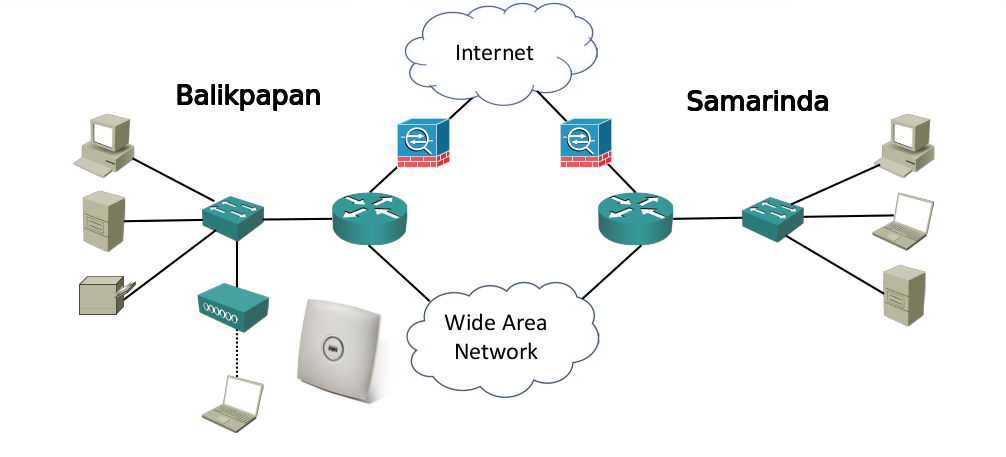
\includegraphics[width=\linewidth]{img/img01}
	\end{center}
\end{frame}

\begin{frame}
	\frametitle{Network Characteristics}
	\begin{itemize}
		\item Topology
		\item Speed
		\item Cost
		\item Security
		\item Availability
		\item Scalability
		\item Reliability
	\end{itemize}
\end{frame}

\section{OSI Model}

\begin{frame}
	\frametitle{OSI Model}
	\begin{itemize}
		\item The OSI reference model is a standard of the International Organization for Standardization (ISO).
		\item It is a general-purpose framework that characterises and standardises how computers communicate with one another over a network.
		\item Its seven-layered approach to data transmission divides the operations into specific related groups of actions at each layer.
		\item A layer serves the layer above it and is served by the layer below it.
	\end{itemize}
\end{frame}

\begin{frame}
	\frametitle{OSI Model - Encapsulation}
	\begin{center}
		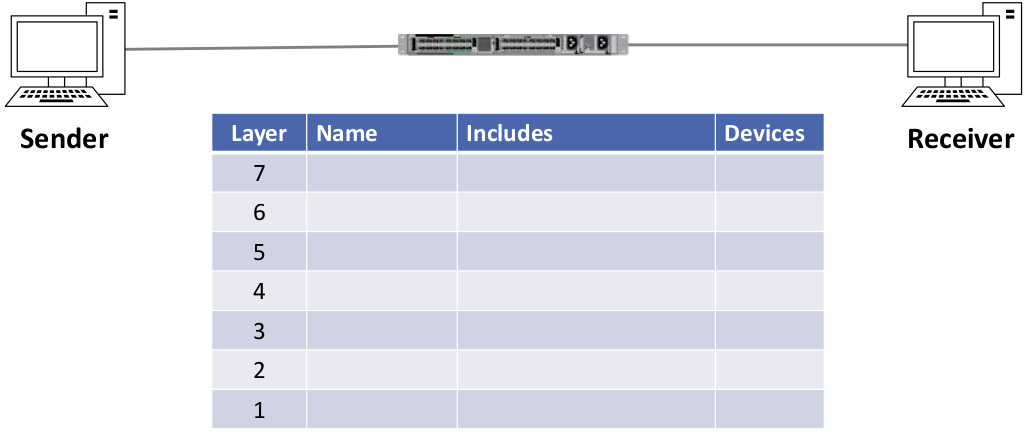
\includegraphics[width=\linewidth]{img/img02}
	\end{center}
\end{frame}

\begin{frame}
	\frametitle{OSI Model - Encapsulation}
	\begin{center}
		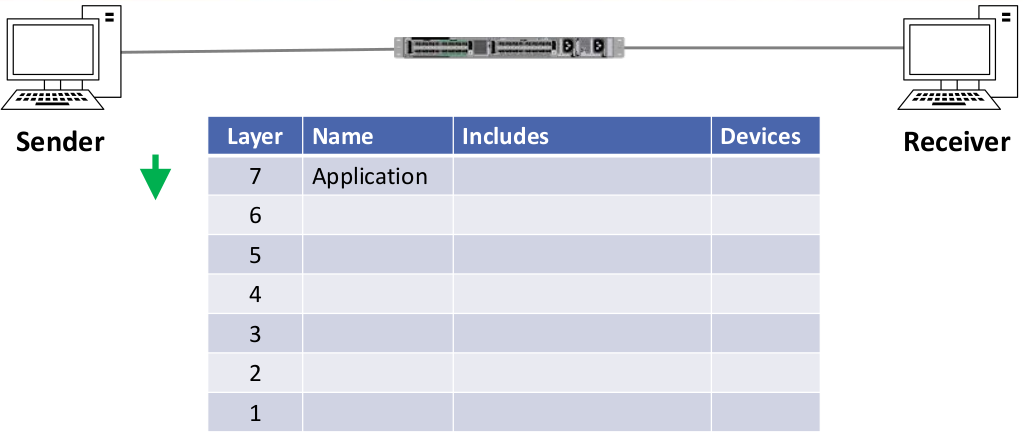
\includegraphics[width=\linewidth]{img/img03}
	\end{center}
\end{frame}

\begin{frame}
	\frametitle{OSI Model - Encapsulation}
	\begin{center}
		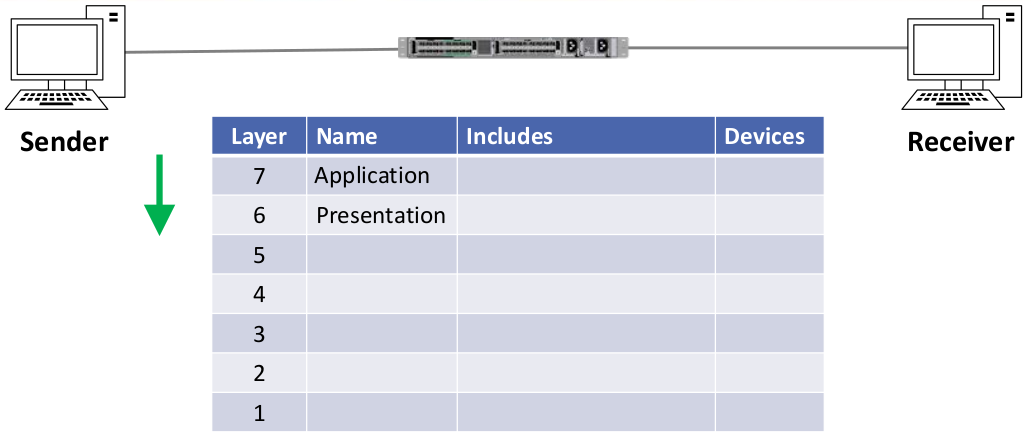
\includegraphics[width=\linewidth]{img/img04}
	\end{center}
\end{frame}

\begin{frame}
	\frametitle{OSI Model - Encapsulation}
	\begin{center}
		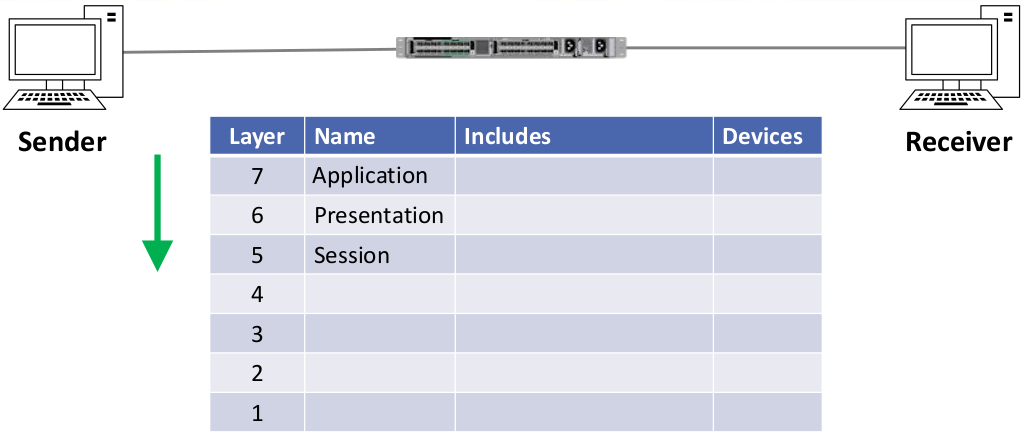
\includegraphics[width=\linewidth]{img/img05}
	\end{center}
\end{frame}

\begin{frame}
	\frametitle{OSI Model - Encapsulation}
	\begin{center}
		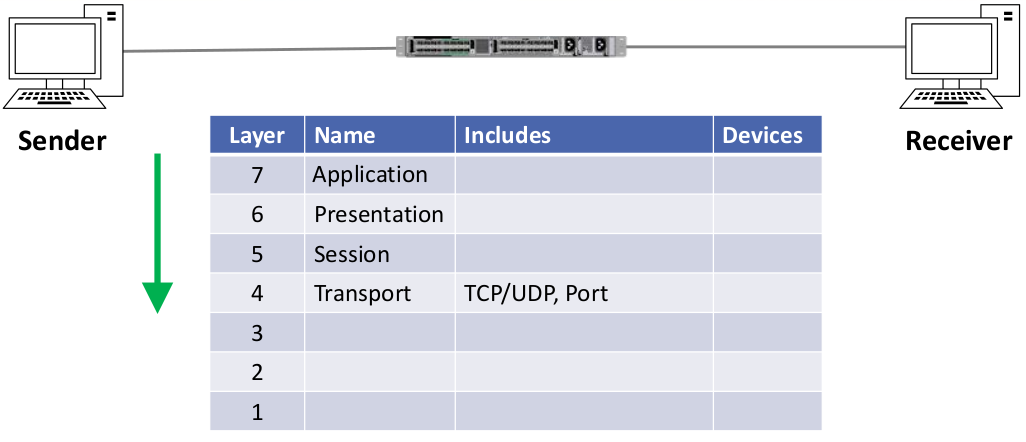
\includegraphics[width=\linewidth]{img/img06}
	\end{center}
\end{frame}

\begin{frame}
	\frametitle{OSI Model - Encapsulation}
	\begin{center}
		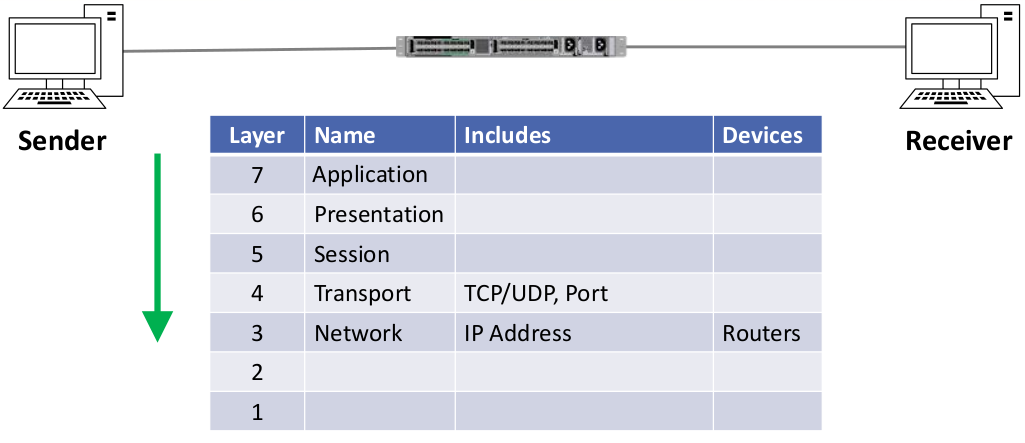
\includegraphics[width=\linewidth]{img/img07}
	\end{center}
\end{frame}

\begin{frame}
	\frametitle{OSI Model - Encapsulation}
	\begin{center}
		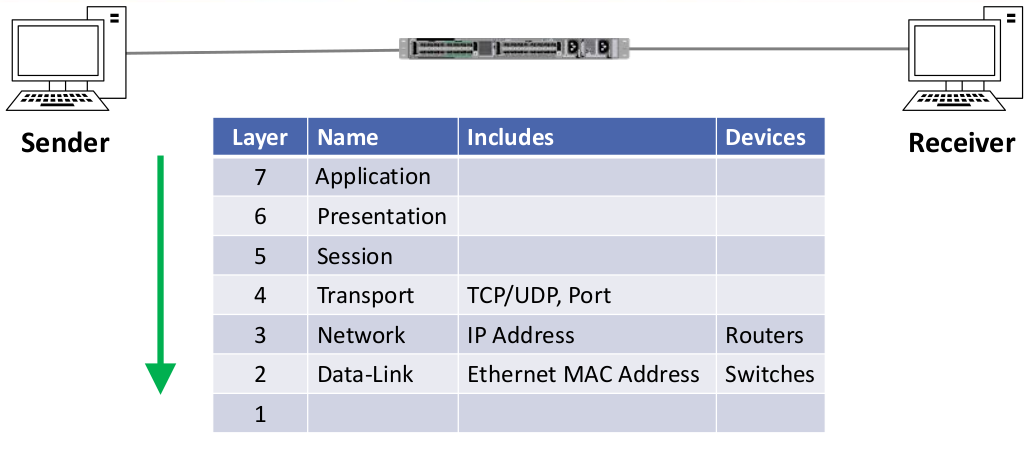
\includegraphics[width=\linewidth]{img/img08}
	\end{center}
\end{frame}

\begin{frame}
	\frametitle{OSI Model - Encapsulation}
	\begin{center}
		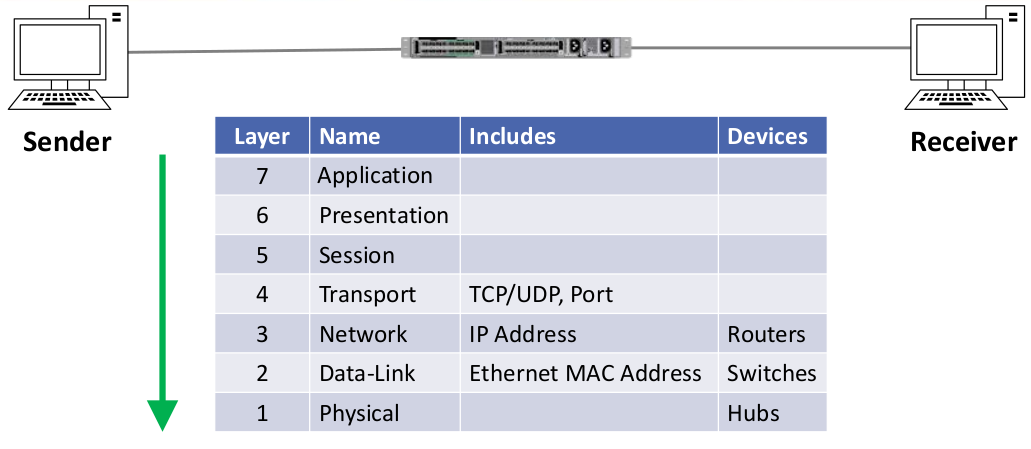
\includegraphics[width=\linewidth]{img/img09}
	\end{center}
\end{frame}

\begin{frame}
	\frametitle{OSI Model - De-encapsulation}
	\begin{center}
		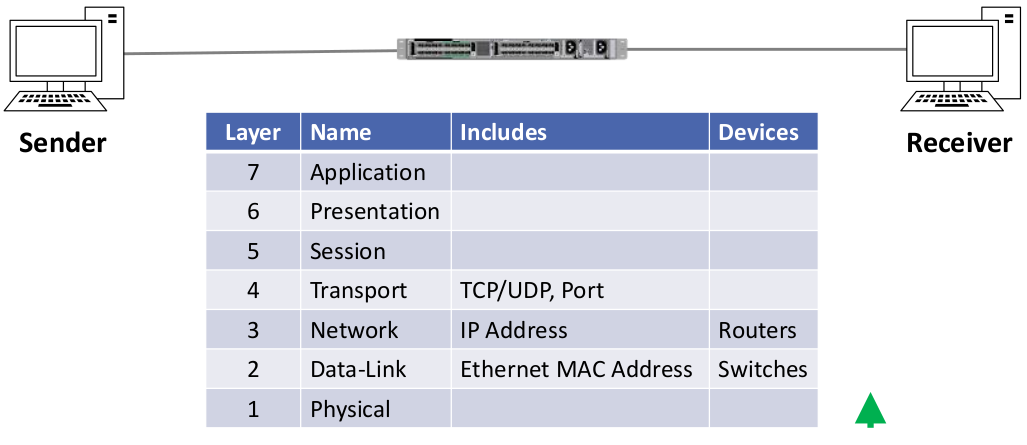
\includegraphics[width=\linewidth]{img/img10}
	\end{center}
\end{frame}

\begin{frame}
	\frametitle{OSI Model - De-encapsulation}
	\begin{center}
		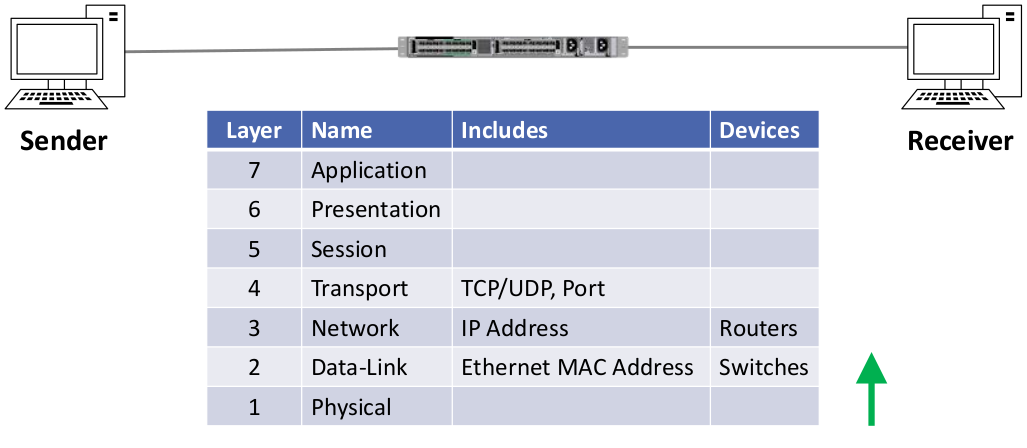
\includegraphics[width=\linewidth]{img/img11}
	\end{center}
\end{frame}

\begin{frame}
	\frametitle{OSI Model - De-encapsulation}
	\begin{center}
		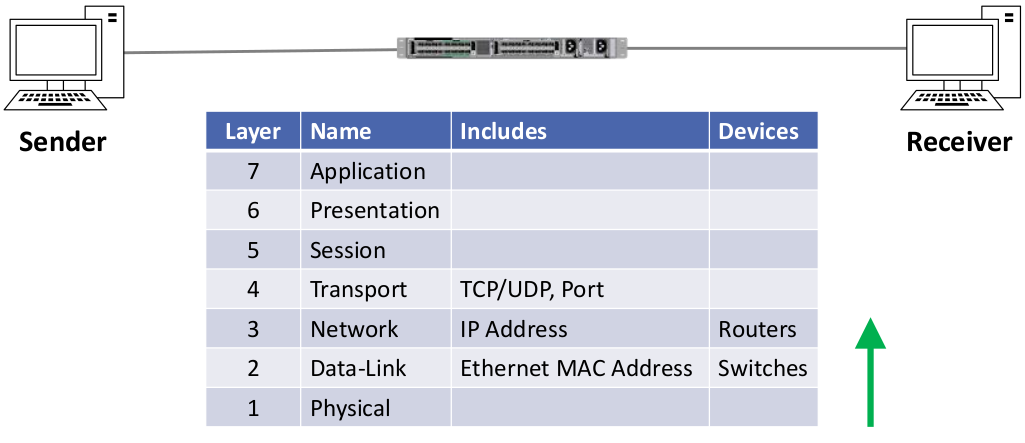
\includegraphics[width=\linewidth]{img/img12}
	\end{center}
\end{frame}

\begin{frame}
	\frametitle{OSI Model - De-encapsulation}
	\begin{center}
		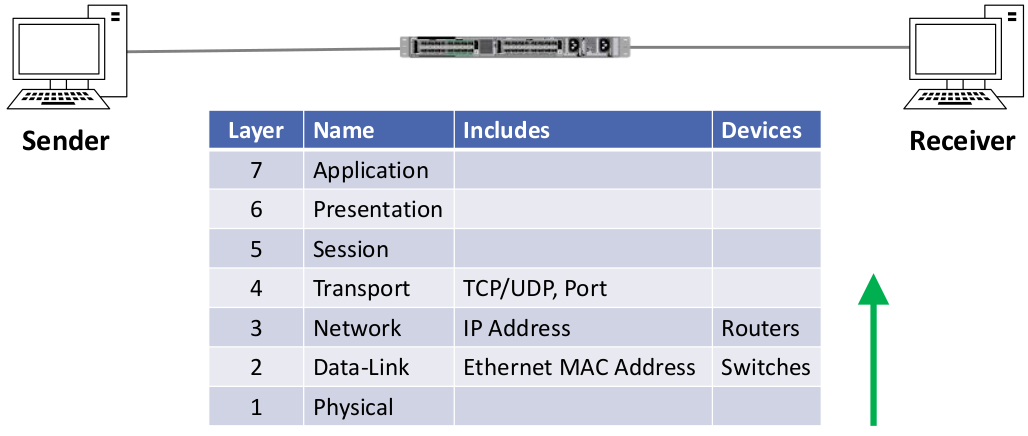
\includegraphics[width=\linewidth]{img/img13}
	\end{center}
\end{frame}

\begin{frame}
	\frametitle{OSI Model - De-encapsulation}
	\begin{center}
		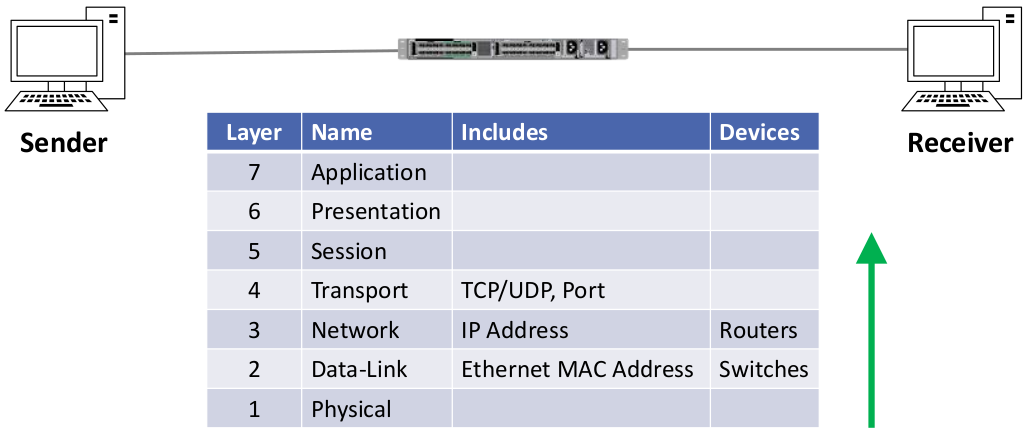
\includegraphics[width=\linewidth]{img/img14}
	\end{center}
\end{frame}

\begin{frame}
	\frametitle{OSI Model - De-encapsulation}
	\begin{center}
		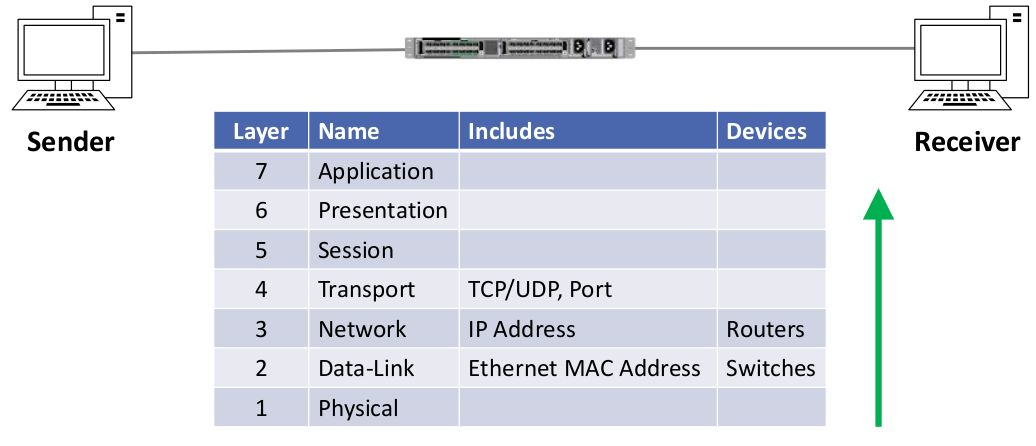
\includegraphics[width=\linewidth]{img/img15}
	\end{center}
\end{frame}

\begin{frame}
	\frametitle{OSI Model - De-encapsulation}
	\begin{center}
		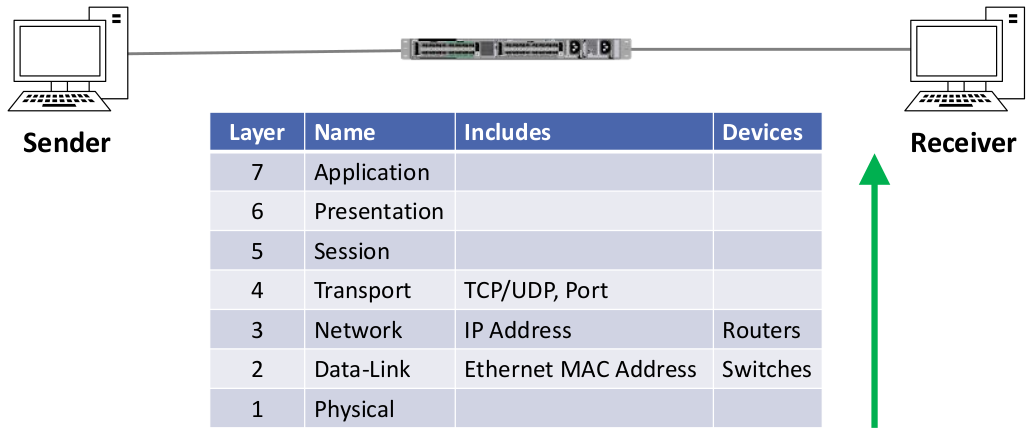
\includegraphics[width=\linewidth]{img/img16}
	\end{center}
\end{frame}

\begin{frame}
	\frametitle{OSI Model Benefits}
	\begin{itemize}
		\item Engineers do not need to design a technology to work end to end from top to bottom of the model. They can just focus on their layer of expertise, and make sure they comply with the standards for the layers above and below.
		\item This leads to open standards and multi-vendor interoperability.
		\item For example: If you’re an application developer, you can just focus on the top three layers, the lower layers are the domain of network engineers.
		\item Troubleshooting is easier because you can analyse a problem in a logical fashion layer by layer.
	\end{itemize}
\end{frame}

\begin{frame}
	\begin{itemize}
		\item It’s difficult to overstate how important the OSI Model is to computer networking.
		\item As you become more experienced you will ‘think’ according to the OSI model when you are troubleshooting or learning a new network technology.
		\item On the job you will hear technologies and problems being described according to their OSI layer.
	\end{itemize}
\end{frame}

\section{The TCP/IP Stack}

\begin{frame}
	\frametitle{The TCP/IP Suite}
	\begin{itemize}
		\item TCP/IP was developed during the 1960s by the US Department of Defense’s (DoD) Advanced Research Projects Agency (ARPA).
		\item It is a protocol stack which consists of multiple protocols including TCP Transmission Control Protocol) and IP (Internet Protocol).
		\item It is the main protocol stack used in computer operations today.
		\item Whereas the OSI Reference Model is conceptual, the TCP/IP stack is used to transfer data in production networks.
		\item TCP/IP is also layered but does not use all of the OSI layers, though the layers are equivalent in operation and function.
	\end{itemize}
\end{frame}

\begin{frame}
	\frametitle{Comparing the OSI Model with the TCP/IP Stack}
	\begin{center}
		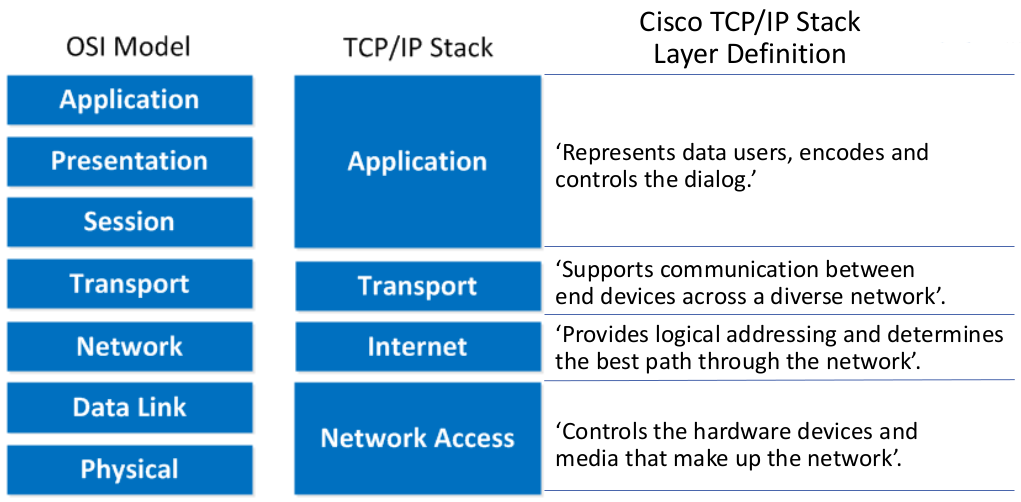
\includegraphics[width=\linewidth]{img/img17}
	\end{center}
\end{frame}

\begin{frame}
	\frametitle{Host Communications Terminology}
	\begin{center}
		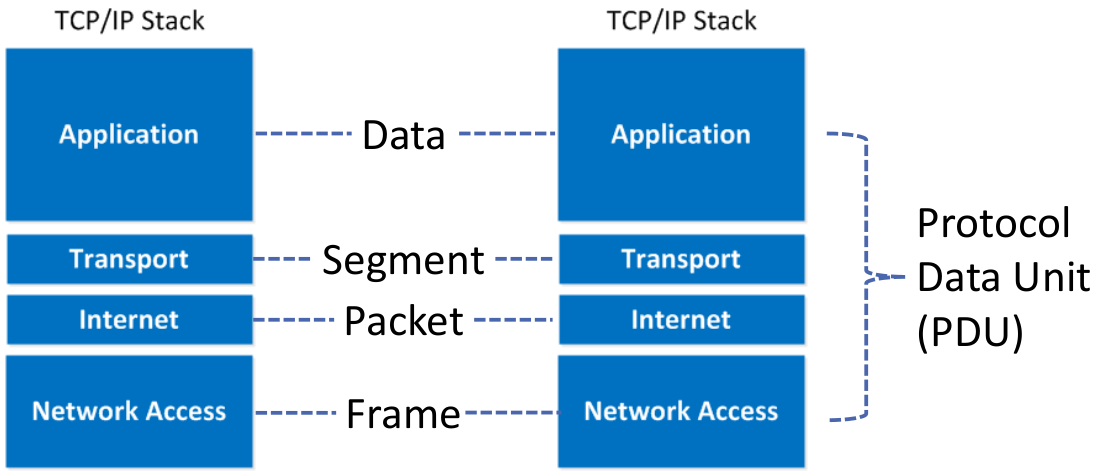
\includegraphics[width=\linewidth]{img/img18}
	\end{center}
\end{frame}

\section{The Upper OSI Layers}

\begin{frame}
	\frametitle{The Upper OSI Layers}
	\begin{itemize}
		\item Network engineers do not typically work directly with the upper 3 layers of the OSI model... but we still need to know what they do.
		\item They are more relevant to application developers.
		\item In this lecture I will primarily be giving you the Cisco definitions of the layers.
		\item Information included in the upper layers would include the Message Body and Subject Line in an email message for example.
	\end{itemize}
\end{frame}

\begin{frame}
	\frametitle{Layer 7 - The Application Layer}
	\begin{itemize}
		\item The application layer provides network services to the applications of the user.
		\item It differs from the other layers in that it does not provide services to any other OSI layer.
		\item The application layer establishes the availability of intended communication partners.
		\item It then synchronizes and establishes agreement on procedures for error recovery and control of data integrity.
	\end{itemize}
\end{frame}

\begin{frame}
	\frametitle{Layer 6 - The Presentation Layer}
	\begin{itemize}
		\item The presentation layer ensures that the information that is sent at the application layer of one system is readable by the application layer of another system.
		\item The presentation layer can translate among multiple data formats using a common format (eg computers with different encoding schemes).
	\end{itemize}
\end{frame}

\begin{frame}
	\frametitle{Layer 5 - The Session Layer}
	\begin{itemize}
		\item The session layer establishes, manages, and terminates sessions between two communicating hosts.
		\item The session layer also synchronizes dialog between the presentation layers of the two hosts and manages their data exchange.
		\item For example, web servers have many users, so there are many communication processes open at any given time to track.
		\item It also offers efficient data transfer, CoS, and exception reporting of upper layer problems.
	\end{itemize}
\end{frame}

\section{The Lower OSI Layers}

\begin{frame}
	\frametitle{The Lower OSI Layers}
	\begin{itemize}
		\item Whereas Network engineers are not particularly interested in the upper OSI layers, we are \textbf{very} concerned with the lower 4 layers of the OSI model.
		Each of these layers have their own dedicated section later and you will learn much more detailed information about them throughout the course.
	\end{itemize}
\end{frame}

\begin{frame}
	\frametitle{Layer 4 - The Transport Layer}
	\begin{itemize}
		\item The main characteristics of the Transport layer are whether TCP or UDP transport is used, and the port number.
		\item Definition:
		\begin{itemize}
			\item The transport layer defines services to segment, transfer, and reassemble the data for individual communications between the end devices.
			\item It breaks down large files into smaller segments that are less likely to incur transmission problems.
		\end{itemize}
	\end{itemize}
\end{frame}

\begin{frame}
	\frametitle{Layer 3 - The Network Layer}
	\begin{itemize}
		\item The most important information at the Network layer is the source and destination IP address.
		\item Routers operate at Layer 3.
		\item Definition:
		\begin{itemize}
			\item The network layer provides connectivity and path selection between two host systems that may be located on geographically separated networks.
			\item The network layer is the layer that manages the connectivity of hosts by providing logical addressing.
		\end{itemize}
	\end{itemize}
\end{frame}

\begin{frame}
	\frametitle{Layer 2 - The Data-Link Layer}
	\begin{itemize}
		\item The most important information at the Data-Link layer is the source and destination layer 2 address.
		\item For example the source and destination MAC address if Ethernet is the layer 2 technology.
		\item Switches operate at Layer 2.
		\item Definition:
		\begin{itemize}
			\item The data link layer defines how data is formatted for transmission and how access to physical media is controlled.
			\item It also typically includes error detection and correction to ensure a reliable delivery of the data.
		\end{itemize}
	\end{itemize}
\end{frame}

\begin{frame}
	\frametitle{Layer 1 - The Physical Layer}
	\begin{itemize}
		\item The Physical layer concerns literally the physical components of the network, for example the cables being used.
		\item Definition:
		\begin{itemize}
			\item The physical link enables bit transmission between end devices.
			\item It defines specifications needed for activating, maintaining, and deactivating the physical link between end devices.
			\item For example, voltage levels, physical data rates, maximum transmission distances, physical connectors etc.
		\end{itemize}
	\end{itemize}
\end{frame}

\begin{frame}
	\begin{center}
		
\includegraphics[width=1\linewidth]{../../img/thank_you}
	\end{center}
\end{frame}

\begin{frame}
	\begin{center}
		
\includegraphics[width=1\linewidth]{../../img/any_questions}
	\end{center}
\end{frame}

\end{document}